Minimum clearance dipilih sebagai indikator utama keselamatan navigasi pada
penelitian ini karena merepresentasikan jarak terdekat yang pernah dicapai
robot terhadap \textit{obstacle} di sepanjang satu \textit{trial}, sesuai
definisi $c_\text{min}$ pada Persamaan~\ref{eq:min_clearance}
(Subbab~\ref{sec:metrik}). Semakin besar nilai minimum clearance, semakin
besar margin keselamatan yang dimiliki robot terhadap kemungkinan tabrakan.
Metrik ini dipilih sebagai variabel utama pengujian hipotesis karena paling
langsung merepresentasikan tujuan rancangan metode usulan, yaitu
\textit{virtual scan} untuk menangani \textit{obstacle} pada area
\textit{blind-spot}, fusi \textit{traversability} termal, dan adaptasi
fuzzy terhadap kondisi lingkungan, yang ketiganya dirancang untuk
memperbesar jarak aman robot terhadap \textit{obstacle}, bukan sekadar
mempercepat waktu tempuh. Meskipun demikian, peningkatan margin keselamatan
pada metode usulan belum dapat disimpulkan sebelum dilakukan analisis
deskriptif dan inferensial secara menyeluruh pada bagian-bagian berikut.

\begin{table}[H]
\centering
\caption{Perbandingan minimum clearance rata-rata antara konfigurasi
\textit{baseline} dan \textit{proposed method} pada keempat pasangan
skenario.}
\label{tab:clearance_deskriptif}
\resizebox{\textwidth}{!}{%
\begin{tabular}{llcccc}
\toprule
\textbf{Pasangan} & \textbf{Lingkungan} & \textbf{Baseline (m)} & \textbf{Proposed (m)} & \textbf{$\Delta$ (m)} & \textbf{\% Increase} \\
\midrule
S1--S5 & Terbuka & 0,000 $\pm$ 0,000 & 0,000 $\pm$ 0,000 & 0,000 & n/a \\
S2--S6 & Obstacle statis tunggal & 0,430 $\pm$ 0,008 & 0,437 $\pm$ 0,000 & +0,007 & 1,6\% \\
S3--S7 & Statis majemuk + kucing & 0,061 $\pm$ 0,001 & 0,182 $\pm$ 0,074 & +0,121 & 198,4\% \\
S4--S8 & Dinamis + kucing & 0,014 $\pm$ 0,092 & 0,317 $\pm$ 0,022 & +0,303 & 2164,3\%$^{*}$ \\
\bottomrule
\end{tabular}%
}
\vspace{1mm}

{\footnotesize $^{*}$Persentase pada S4--S8 sangat besar karena rata-rata
\textit{baseline} mendekati nol; nilai selisih absolut ($\Delta$) lebih
representatif untuk dibaca pada pasangan ini dibandingkan persentase.}
\end{table}

\begin{figure}[H]
\centering
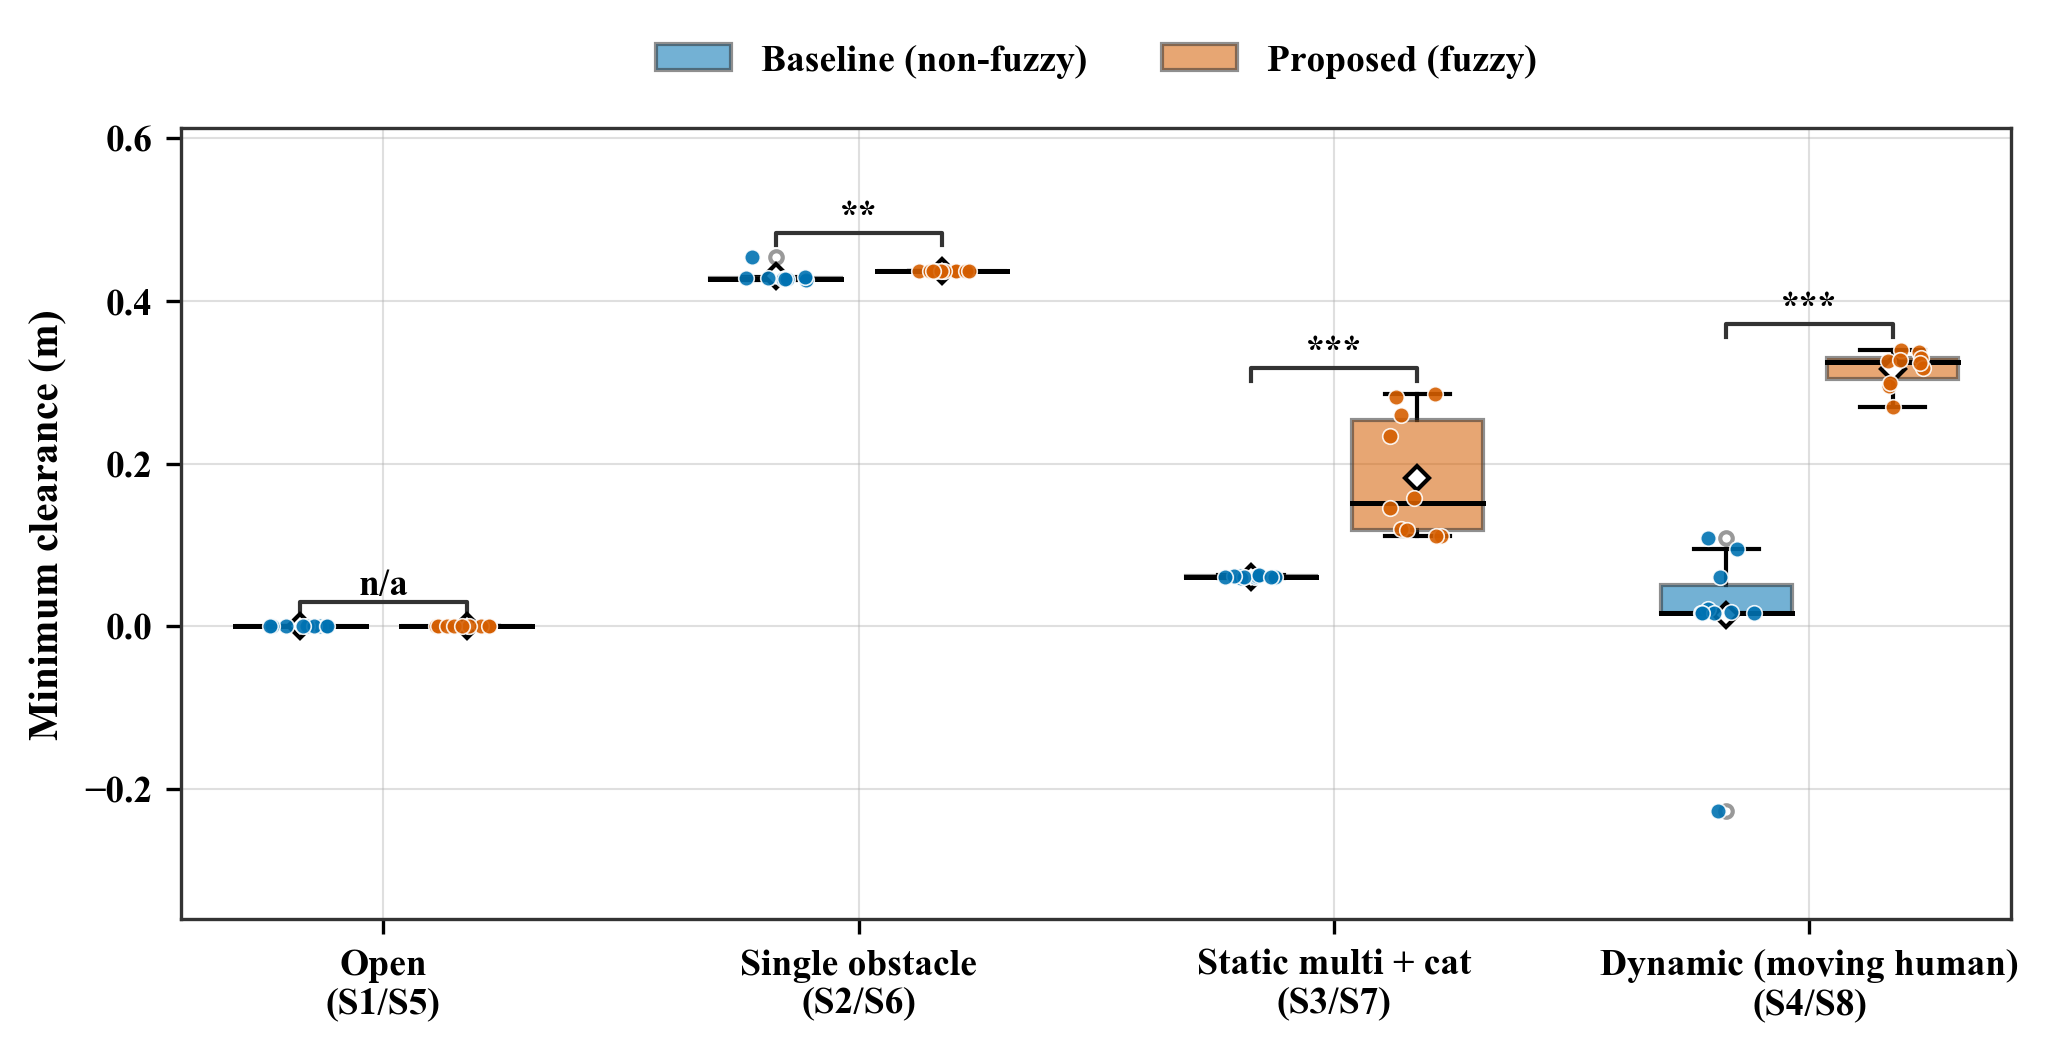
\includegraphics[width=0.9\textwidth]{gambar/4.4_clearance_boxplot.png}
\caption{\textit{Boxplot} minimum clearance berpasangan (\textit{baseline}
vs.\ \textit{proposed method}) per lingkungan pengujian, disertai titik data
individual dan simbol signifikansi hasil uji Mann-Whitney U.}
\label{fig:clearance_boxplot}
\end{figure}

Tabel~\ref{tab:clearance_deskriptif} dan Gambar~\ref{fig:clearance_boxplot}
menunjukkan empat pola yang berbeda pada keempat pasangan skenario. Pada
S1/S5, kedua konfigurasi sama-sama menghasilkan minimum clearance 0,000~m
tanpa perbedaan, sesuai dengan tidak adanya \textit{obstacle} aktif pada
lingkungan terbuka ini. Pada S2/S6, terdapat peningkatan kecil pada
konfigurasi \textit{proposed method} (+0,007~m). Pada S3/S7, peningkatan
tampak lebih jelas (+0,121~m), sementara peningkatan paling besar secara
absolut ditemukan pada S4/S8 (+0,303~m), termasuk satu titik data ekstrem
pada \textit{baseline} S4 yang mencatat clearance negatif ($-0,227$~m),
konsisten dengan kejadian tabrakan tunggal yang telah dibahas pada
Subbab~\ref{sec:keberhasilan_tabrakan}.

Perbedaan minimum clearance antara kedua konfigurasi pada setiap pasangan
diuji menggunakan uji Mann-Whitney U, sesuai metode yang telah ditetapkan
pada Subbab~\ref{sec:metode_statistik}. Uji non-parametrik dipilih karena
distribusi clearance umumnya tidak simetris akibat adanya batas bawah fisik
dan ukuran sampel yang kecil ($n=10$ per kelompok). Hipotesis yang diuji
untuk setiap pasangan adalah:
\begin{itemize}
    \item $H_0$: tidak terdapat perbedaan distribusi minimum clearance
    antara konfigurasi \textit{baseline} dan \textit{proposed method}.
    \item $H_1$: terdapat perbedaan distribusi minimum clearance antara
    kedua konfigurasi (uji dua arah).
\end{itemize}

\begin{table}[H]
\centering
\caption{Hasil uji Mann-Whitney U untuk minimum clearance pada keempat
pasangan skenario ($\alpha=0,05$).}
\label{tab:clearance_mwu}
\begin{tabular}{lccc}
\toprule
\textbf{Pasangan} & \textbf{$U$} & \textbf{$p$} & \textbf{Signifikan} \\
\midrule
S1--S5 & n/a & n/a & n/a \\
S2--S6 & 10 & 0,0013 & ** \\
S3--S7 & 0 & 0,0002 & *** \\
S4--S8 & 0 & 0,0002 & *** \\
\bottomrule
\end{tabular}
\end{table}

Pada pasangan S1/S5, uji tidak dapat dilakukan karena kedua kelompok
bernilai konstan dan identik (0,000~m pada seluruh 10 \textit{trial} di
kedua konfigurasi), sehingga distribusi tidak memiliki variansi yang
diperlukan agar uji Mann-Whitney U terdefinisi; hasil ditandai n/a pada
Tabel~\ref{tab:clearance_mwu}, konsisten dengan anotasi yang sama pada
Gambar~\ref{fig:clearance_boxplot}. Pada ketiga pasangan lainnya, uji
menunjukkan perbedaan yang signifikan secara statistik pada $\alpha=0,05$
($p=0,0013$ untuk S2/S6; $p=0,0002$ untuk S3/S7 dan S4/S8), sehingga $H_0$
ditolak untuk ketiga pasangan tersebut.

Signifikansi statistik semata tidak cukup untuk menyimpulkan kuat tidaknya
perbedaan, terutama pada ukuran sampel kecil, sehingga besaran perbedaan
dihitung menggunakan \textit{effect size rank-biserial correlation} $r$
sesuai Persamaan~\ref{eq:rank_biserial}.

\begin{table}[H]
\centering
\caption{Effect size (\textit{rank-biserial correlation}) untuk minimum
clearance pada keempat pasangan skenario.}
\label{tab:clearance_effect_size}
\begin{tabular}{lcc}
\toprule
\textbf{Pasangan} & \textbf{Effect Size ($r$)} & \textbf{Interpretasi} \\
\midrule
S1--S5 & n/a & n/a \\
S2--S6 & +0,80 & Besar \\
S3--S7 & +1,00 & Besar \\
S4--S8 & +1,00 & Besar \\
\bottomrule
\end{tabular}
\end{table}

Pada ketiga pasangan yang signifikan, nilai $r$ bertanda positif, yang pada
metrik minimum clearance berarti konfigurasi \textit{proposed method}
secara konsisten menghasilkan nilai clearance yang lebih besar dibandingkan
\textit{baseline}. Berdasarkan kriteria pada Tabel~\ref{tab:effect_size}
(Subbab~\ref{sec:metode_statistik}), ketiga effect size tersebut tergolong
\textit{besar} ($|r| \geq 0,50$), menunjukkan bahwa perbedaan yang teramati
bukan hanya signifikan secara statistik, tetapi juga substansial secara
praktis.

Secara keseluruhan, peningkatan minimum clearance paling nyata terjadi pada
skenario yang melibatkan kondisi \textit{blind-spot} dan \textit{obstacle}
dinamis (S3/S7 dan S4/S8), yaitu kondisi yang paling dekat dengan tujuan
rancangan metode usulan. Temuan pada S3/S7 secara khusus menjawab
pertanyaan utama penelitian yang telah dirumuskan pada
Subbab~\ref{sec:interpretasi}, yaitu apakah konfigurasi fuzzy secara
signifikan meningkatkan clearance minimum dibandingkan \textit{baseline}
pada skenario dengan \textit{obstacle} kucing. Hasil pada pasangan ini
($p=0,0002$; $r=+1,00$) mendukung hipotesis tersebut. Meskipun demikian,
pola peningkatan tidak seragam di seluruh skenario: pada S1/S5 tidak
terdapat perbedaan sama sekali, sedangkan pada S2/S6 peningkatan tergolong
kecil secara absolut (+0,007~m) meskipun signifikan secara statistik.
Dengan demikian, peningkatan margin keselamatan oleh metode usulan tidak
dapat digeneralisasi berlaku sama besar pada seluruh kondisi lingkungan,
melainkan tampak paling bermanfaat pada kondisi yang memang dirancang untuk
ditangani oleh komponen-komponen metode usulan.

Pola hasil di atas konsisten dengan kontribusi yang diharapkan dari ketiga
komponen utama metode usulan. \textit{Virtual scan} untuk area
\textit{blind-spot} relevan terutama pada S3/S7, tempat kucing berada pada
posisi yang tidak terjangkau LiDAR; fusi \textit{traversability} termal
berkontribusi pada deteksi \textit{obstacle} bersuhu rendah seperti kucing
di kedua konfigurasi, namun pemanfaatannya lebih komprehensif pada
konfigurasi fuzzy; sementara adaptasi fuzzy terhadap kecepatan dan
penguatan repulsi relevan pada seluruh skenario dengan \textit{obstacle},
termasuk S4/S8. Karena penelitian ini tidak melakukan eksperimen
\textit{ablation} yang menonaktifkan masing-masing komponen secara
independen, kontribusi relatif ketiga komponen tersebut terhadap
peningkatan minimum clearance tidak dapat dipisahkan satu sama lain; yang
dapat disimpulkan secara valid adalah bahwa kombinasi ketiganya, sebagai
satu kesatuan metode usulan, secara empiris meningkatkan margin keselamatan
dibandingkan \textit{baseline} pada skenario yang relevan.

Beberapa keterbatasan perlu dicatat dalam membaca hasil ini. Pertama, nilai
minimum clearance bergantung pada konfigurasi parameter simulator Gazebo,
termasuk dimensi \textit{obstacle} dan mekanisme deteksi tabrakan
\textit{ground-truth} yang telah dijelaskan pada
Subbab~\ref{sec:perangkat_keras}, sehingga nilai absolut dapat berbeda pada
konfigurasi simulasi lain. Kedua, jumlah \textit{trial} per skenario
($n=10$) tergolong kecil untuk standar statistik umum, meskipun hal ini
telah dipertimbangkan melalui pemilihan uji non-parametrik dan pelaporan
effect size. Ketiga, seluruh hasil diperoleh dari simulasi dan belum
divalidasi pada robot fisik, sehingga generalisasi terhadap kondisi dunia
nyata, misalnya noise sensor atau dinamika kontak aktual, masih memerlukan
pengujian lebih lanjut.

Setelah mengevaluasi aspek keselamatan melalui minimum clearance, analisis
selanjutnya membahas \textit{trade-off} performa yang menyertainya, khususnya
melalui waktu tempuh dan efisiensi lintasan, yang disajikan pada Subbab 4.5.